\documentclass[UTF8]{article}
\usepackage{graphicx}
%--
\usepackage{ctex}
\usepackage[margin=1in]{geometry}

%--
\begin{document}
    
%--
{\flushleft \bf \Large 姓名:} 杨佩成

{\flushleft \bf \Large 学号:} MG1733079

{\flushleft \bf \Large 日期:} 2018.1.12


%=========================================================================
\section*{论文信息}
    
Decandia G, Hastorun D, Jampani M, et al. Dynamo: amazon's highly available key-value store[C]// ACM Sigops Symposium on Operating Systems Principles. ACM, 2007:205-220.
    
%=========================================================================
\section{章节1}
	Dynamo是Amazon设计的高可用性的键值存储系统。Amazon使用了一个高度分散、松耦合和面向服务的架构,在这种环境下,存储系统需要一直保持可用。Amazon的基础设施由上百万的组件构成,服务器错误和网络组件错误是经常出现的,Dynamo需要在保证系统可用性和性能的同时应对各种错误的发生。Dynamo还需要有高度可扩展性,通过增加节点实现容量和性能的线性扩展。除此之外,Dynamo的设计还需要满足以下要求和假设:
\begin{itemize}

	\item
		查询模型:一条数据可以用一个唯一的Key来确定,没有跨越多条数据的操作和关系模型。Dynamo所面向应用存储的数据很小,通常小于1MB。
	\item
           ACID属性:ACID是一组保证数据库正确运行的属性,但是保证ACID会损失系统的可用性。Dynamo弱化了一致性的要求而希望提高可用性。Dynamo不提供隔离性保证,只允许单条数据的更新。
	\item
           效率:系统的延迟要满足SLA(Service Level Agreement),服务可以根据自己的要求配置Dynamo。
	\item
           其它假设:Dynamo只在Amazon内部使用,所以没有安全上的要求。每个服务运行一个Dynamo的实例,要保证系统的可扩展性。
		
\end{itemize}
%--    


%=========================================================================
\section{系统架构}
	\subsection{系统接口}
		Dynamo通过一个简单的接口来存储与一个Key关联的对象,接口提供了get和put操作。get(key)会返回key对应的对象,如果副本之间没有冲突,会返回单个对象;否则,会返回一组发生冲突的副本和它对应的context,交给应用处理。

	\subsection{数据分布}
		Dynamo的一个关键需求是它必须可扩展,这需要一个能在系统节点上动态划分数据的机制。Dynamo使用了一致性哈希算法将数据分布到多台存储主机上。在一致性哈希算法中,hash函数的输出值为一个ring。系统中的每一个节点分配一个随机数,代表了它在ring上的位置。每个数据项通过对它的key做hash运算,得到它在ring上的位置,然后沿顺时针找到第一个节点。每个节点负责ring上它和后继节点之间的区域。一致性哈希算法的主要优势是节点的加入和离开只会影响它的邻居节点,不会影响其它节点。

		基本的一致性哈希算法可能会导致不均匀的数据和负载分配,另外它也没有考虑到异构节点之间性能的差异。Dynamo使用了一致性哈希算法的一种变体,它使用了虚拟节点的概念。一个虚拟节点对应ring上的一个位置,而一个物理节点对应多个虚拟节点。定位时,首先根据key计算得到数据所在的虚拟节点,再通过查表知道虚拟节点对应的物理节点,这相当于是一个二级映射。使用虚拟节点带来的好处是:
		\begin{itemize}
			\item
				当一个节点不可用时,由该节点处理的负载会被均匀分布到其它可用节点上。
			\item
                     当一个节点重新恢复或者一个新的节点加入系统时,新的可用节点会接受与其它节点大致相同的负载。
                \item
                     一个物理节点对应虚拟节点的数量,可以根据它的性能来决定。
		\end{itemize}
	
	\subsection{数据复制与一致性}
		为了保证系统的高可用性和持久性,Dynamo会将数据在N台主机上备份,N是一个可以配置的参数。每一个key会被分配给一个协作节点,协作节点除了会在本地存储数据,还会通知另外的N-1个节点复制该数据。负责存储指定key的节点列表被称为优先列表。考虑到节点可能失效,优先列表会包含大于N的节点。因为使用了虚拟节点,所以N个后继节点可能分配在小于N的物理节点上。为了解决这个问题,优先列表会在ring上跳过位置来构建,以确保列表中的节点不在同一个物理节点上。

		由于系统使用了多个副本,所以需要考虑副本之间的一致性问题。Dynamo使用的是最终一致性模型:多个副本之间可能会存在不一致的时间窗口,但是最终系统会保证副本之间的数据达成一致。Dynamo将每次数据修改后的结果作为新的、不可变的数据版本,这就允许系统中同时存在一个对象的多个版本。大部分情况下,新版本的数据会包含旧的版本,系统会自动判断权威版本的数据。但是当出现故障或者并行更新时,一个对象可能会有多个冲突的数据版本。在这种情况下,系统不能够在多个版本中达成一致,只能交给客户端来合并不同版本的数据。

		Dynamo使用向量时钟来确定同一对象不同版本之间的因果关系。向量时钟是一组$<$节点,计数器$>$对。通过比较不同数据版本的向量时钟,可以判断两个版本是在并行的分支上,还是存在因果顺序关系。如果一个对象的时钟计数器小于等于另一个对象在所有节点上的时钟计数器,那第一个对象就是第二个对象的祖先,可以被丢弃。否则,两者之间就存在冲突。当客户端更新对象时,它必须指定要更新的版本,这通过上次读操作获取的context信息确定(context信息中包括了向量时钟信息)。当客户端需要读取数据时,如果Dynamo因为有多个数据版本分支而存在冲突,它会返回所有冲突数据,客户端程序会根据自己的业务逻辑去解决冲突。然后客户端会将自己的协调结果写回,冲突的数据就会通过协调达成一致。

		Dynamo使用了基于多数表决的一致性协议,协议包括了两个参数R和W。R是读成功需要参与的最少节点数量,W是写成功需要参与的最少节点数量,R+W$>$N。读写操作的延迟由最慢的副本决定,所以通常设置R和W小于N以降低延迟。当收到put请求时,只有当W个节点完成操作后,写请求才会被认为成功完成,get请求也类似。如果应用想要达到最高级别的可用性,会将W设为1。这样只有当系统中的所有节点都不能被访问时,请求才会被拒绝。在Dynamo中,通常会将W设得更高些,以保证系统的持久性。

	\subsection{故障处理}
		当出现网络故障或者服务器故障时,使用传统的基于多数表决的方法会导致系统变得不可用。为了解决这种问题,Dynamo会使用优先列表中的前N个健康节点,而不总是前N个节点。如图1所示,N=3。如果在写操作时,节点A暂时宕机或者不可访问,A上的备份就会被发送到节点D上。发送到D上的副本在元数据中包含hint,指明副本的预期接收者。接收到包含hinted副本的节点,会周期性的扫描本地数据库,一旦发现A恢复,D就会尝试将副本发送给A。如果发送成功,D就会删除本地的备份。通过这种方式,Dynamo可以保证当发生临时的节点或网络故障时,读写操作不会失效。
\begin{figure}[!h]
\centering
\small
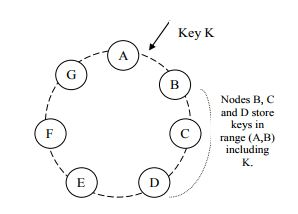
\includegraphics{1.JPG}
\caption{System structure}
\end{figure}
		
上述算法在系统成员流动性低,节点短暂失效的情况下有效。有些情况下,在hinted副本移交回原来副本之前,hinted副本会变得不可用。为了处理这样的情况以及其它持久性的故障,需要保证副本之间的一致性,如果发现不一致,需要进行副本同步。Dynamo使用Merkle Tree来检测副本是否一致。Merkle Tree的主要优点是可以独立地检查每个分支的节点而不需要下载整个数据集。此外,在检测副本一致性时,Merkle Tree只需要传输少量的数据。如果两个树的根hash值相同,树的叶节点就是相同的,主机间就不需要进行同步。如果树的根hash值不同,主机就需要交换children hash值,直到到达树的叶子,这样主机就能确认不同步的key。在Dynamo系统中,每个主机节点为它负责的区域维护一个Merkle Tree,通过上面的方案判断是否需要进行同步。

	\subsection{成员管理与故障检测}
		在Amazon的环境中,节点失效通常是瞬时的,但是也可能会持续多个时间间隔。节点失效很少意味着节点永久离开,因此不应导致数据分布的再平衡和不可访问副本的修复。所以Dynamo使用了明确的机制来初始化节点的加入和删除。管理员连接到Dynamo节点提交一个成员变化请求,来添加或删除ring中的节点。收到请求的节点会将成员变化信息保存到本地磁盘上,并使用基于gossip的协议传播成员变化信息,最终所有节点会达到一致的成员信息视图。当一个节点第一次启动时,它会选择一组虚拟节点的Token,生成一个物理节点到虚拟节点的映射表,映射表会存储在本地磁盘中。节点在交换成员信息的同时交换映射表信息,这样每个节点就会知道它要处理的虚拟节点范围。
		
		由于基于gossip的协议需要一定时间才能实现同步,节点可能会不知道其它节点的存在,所以上面的方案可能会导致ring发生逻辑分裂。因此,Dynamo中引入Seed节点,Seed是通过外部机制发现的节点,并且所有节点都知道Seed节点的存在。因为所有节点的成员信息都会与Seed节点达成一致,所以不会发生逻辑分裂的情况。
		
		为了避免无效的通信请求,Dynamo使用了简单的故障检测机制:如果节点B没有响应节点A的消息,节点A就认为节点B失效。当存在稳定的客户端请求时,节点B失效时,节点A可以很快发现。然后A会使用替代节点来接管B负责的虚拟节点,同时A会周期性的重连B,以检测B是否恢复。当没有客户端请求需要两个节点通信时,节点就不需要知道对方是否失效。通过成员管理信息的交换,持久的节点增加和删除消息会通知给所有的节点。短时的节点失效可以通过节点通信失败来检测。

		当一个新的物理节点加入系统时,它会被分配一组ring上的虚拟节点。而原先负责这些虚拟节点的物理节点将不再存储对应信息,它们会将对应的Key转交给新的节点。当一个物理节点从系统中删除时,Key的分配会按照一个相反的过程。通过这种方法,Dynamo可以将Key的负载均匀地分配给各个节点,这样可以满足延迟的需求并且可以保证节点能迅速启动。		
		

\section{系统实现}
	Dynamo中的每个节点主要由三部分组成:请求协调器,成员管理和错误检测,存储引擎。
	存储引擎使用了模块化设计,支持插拔,支持BDB、MySQL等数据库。
	请求协调器以事件驱动通信为基础,其中消息处理管道使用了类似于SEDA的结构。协调节点代表客户端在一个或多个节点上执行读写操作。每个客户请求会让收到请求的节点创建一个状态机,来执行客户端的请求。如果每次都使用优先列表中的第一个节点作为协调节点,会导致它的负载过大。所以Dynamo会使用优先列表中最先响应的节点作为协调节点。

\section{总结}
	Dynamo是Amazon提出的一种NoSQL数据库,它使用了简单的键值对存储方式。



%--
\end{document}